\documentclass[12pt]{article}

\usepackage[english]{babel}
\usepackage[utf8]{inputenc}
\usepackage{sansmathfonts}
\usepackage[T1]{fontenc}
\renewcommand*\familydefault{\sfdefault} %% Only if the base font of the document is to be sans serif
\usepackage{multicol,lipsum}
\usepackage{amsmath,cancel}
\usepackage{amssymb,amsthm,dsfont,mathrsfs}
\usepackage[colorinlistoftodos]{todonotes}
\usepackage{geometry}
\geometry{
a4paper,
total={170mm,257mm},
left=20mm,
top=15mm,
bottom=22mm,
}
\usepackage{natbib}
\usepackage{soul}
\usepackage{setspace}
\usepackage{hyperref}
\usepackage{xcolor}
\usepackage{graphicx}
\usepackage{tikz}
\usepackage{siunitx}
\graphicspath{ {imagens/} }
\usepackage{fancyhdr}
\pagestyle{fancy}
\renewcommand{\headrulewidth}{0pt}

\color{darkgray}
\newcommand{\T}[1]{\vspace{0.4cm}\textbf{\large#1}}
\newcommand{\TW}[1]{\textbf{\large#1}}

\newcommand{\TM}[1]{\vspace{0.2cm} \textbf{#1}}

\newcommand{\M}[1]{
\vspace{-0.6cm}
\begin{flalign*}
#1&
\end{flalign*}
\vspace{-0.6cm}
}


\definecolor{bluebell}{rgb}{0.25, 0.35, 0.89} 
\definecolor{laranja}{rgb}{0.87, 0.48, 0.25} 
\definecolor{verde}{rgb}{0, 0.54, 0.44} 
\definecolor{babypink}{rgb}{1, 0.42, 0.52} 
\definecolor{rosa}{rgb}{1, 0.72, 0.77} 
\definecolor{cinza}{rgb}{0.3, 0.3, 0.3}  
\definecolor{iris}{rgb}{0.25, 0.35, 0.89}  
\definecolor{babyblue}{rgb}{0.13, 0.59, 0.95}

\setlength\columnsep{30pt}

\setlength{\parindent}{0cm}
\setlength{\fboxrule}{1.3pt}  % <-- Aumenta a espessura

\newcommand{\Formula}[1]{
\begin{center}
\color{iris}
\fcolorbox{rosa}{white}{
\(
\begin{array}{c}
#1
\end{array}
\)
}
\color{cinza}
\end{center}
}

\begin{document}
\pagenumbering{gobble}
\setstretch{1.3}


\includegraphics[width=4cm]{Logo2.png}
\begin{center}
    \textbf{\Huge \textcolor{bluebell}{Ângulo Inscrito na Circunferência}}
\end{center}

\begin{multicols}{2}

\TW{Definição} 

O ângulo inscrito na circunferência é um ângulo cujo vértice está sobre a circunferência e seus lados são segmentos de reta que interceptam a circunferência em dois pontos diferentes.

A principal característica do ângulo inscrito é que ele é sempre metade do ângulo central que subtende o mesmo arco da circunferência. Geometricamente, isso ocorre porque o triângulo formado pelo centro e pelos dois pontos do arco é isósceles (lados iguais ao raio), e o ângulo externo do vértice inscrito é igual à soma dos dois ângulos da base — exatamente o dobro do ângulo inscrito.

Se $\beta$ for o ângulo inscrito e $\alpha$ for o ângulo central que subtende o mesmo arco, então:

\Formula{
\beta = \dfrac{\alpha}{2} \quad \Longleftrightarrow \quad \alpha = 2\,\beta
}

\begin{center}
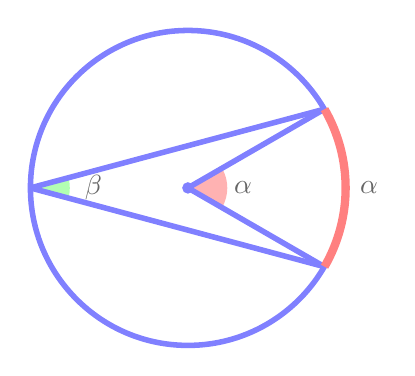
\begin{tikzpicture}
\tikzstyle{texto}=[draw=none,fill=none,black!60!white]
\tikzstyle{line}=[blue!50!white,line width=2pt]
\tikzstyle{line2}=[red!50!white,line width=3pt]
\tikzstyle{angleA}=[draw=none,fill=red!30!white]
\tikzstyle{angleB}=[draw=none,fill=green!30!white]

\draw[angleA] (0,0) -- (-30:0.5) arc (-30:30:0.5);

\begin{scope}[shift={(-2,0)}]
    \draw[angleB] (0,0) -- (-15:0.5) arc (-15:15:0.5);
\end{scope}

\draw[line] (0,0) -- (30:2) (0,0) -- (-30:2);
\draw[line] (-2,0) -- (30:2) (-2,0) -- (-30:2) ;

\filldraw [line] (0,0) circle (1pt);
\draw[line] (0,0) circle (2);

\begin{scope}[shift={(1.735,-1)}]
    \draw[line2] (0,0) arc (-30:30:2);
\end{scope}

\node[texto] at (0.7,0) {\textbf{$\alpha$}};
\node[texto] at (2.3,0) {\textbf{$\alpha$}};
\node[texto] at (-1.2,0) {\textbf{$\beta$}};
\end{tikzpicture}
\end{center}

\TM{Exemplos:}

\begin{center}
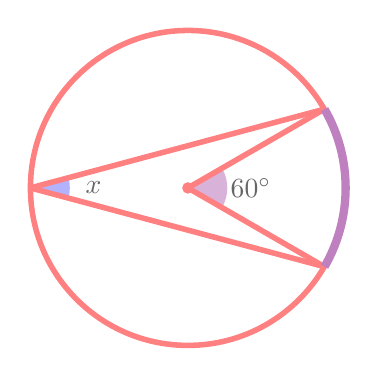
\begin{tikzpicture}
\tikzstyle{texto}=[draw=none,fill=none,black!60!white]
\tikzstyle{line}=[red!50!white,line width=2pt]
\tikzstyle{line2}=[violet!50!white,line width=3pt]
\tikzstyle{angleA}=[draw=none,fill=violet!30!white]
\tikzstyle{angleB}=[draw=none,fill=blue!30!white]

\draw[angleA] (0,0) -- (-30:0.5) arc (-30:30:0.5);

\begin{scope}[shift={(-2,0)}]
    \draw[angleB] (0,0) -- (-15:0.5) arc (-15:15:0.5);
\end{scope}

\draw[line] (0,0) -- (30:2) (0,0) -- (-30:2);
\draw[line] (-2,0) -- (30:2) (-2,0) -- (-30:2) ;

\filldraw [line] (0,0) circle (1pt);
\draw[line] (0,0) circle (2);

\begin{scope}[shift={(1.735,-1)}]
    \draw[line2] (0,0) arc (-30:30:2);
\end{scope}

\node[texto] at (0.8,0) {\textbf{$\ang{60}$}};
\node[texto] at (-1.2,0) {\textbf{$x$}};
\end{tikzpicture}
\end{center}

\vspace{8px}
$x = \dfrac{60}{2}$ \vspace{8px}

$x= 30$


\begin{center}
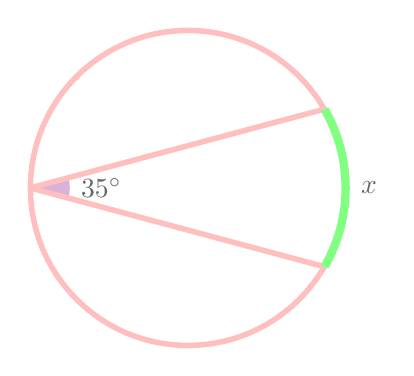
\begin{tikzpicture}
\tikzstyle{texto}=[draw=none,fill=none,black!60!white]
\tikzstyle{line}=[pink,line width=2pt]
\tikzstyle{line2}=[green!50!white,line width=3pt]
\tikzstyle{angleA}=[draw=none,fill=green!30!white]
\tikzstyle{angleB}=[draw=none,fill=violet!30!white]

\begin{scope}[shift={(-2,0)}]
    \draw[angleB] (0,0) -- (-15:0.5) arc (-15:15:0.5);
\end{scope}

\draw[line] (-2,0) -- (30:2) (-2,0) -- (-30:2) ;

\draw[line] (0,0) circle (2);

\begin{scope}[shift={(1.735,-1)}]
    \draw[line2] (0,0) arc (-30:30:2);
\end{scope}

\node[texto] at (2.3,0) {\textbf{$x$}};
\node[texto] at (-1.1,0) {\textbf{$\ang{35}$}};
\end{tikzpicture}
\end{center}

\vspace{8px}
$35 = \dfrac{x}{2}$ \vspace{8px}

$x = 35 \cdot 2$

$x = 70$

\T{Propriedades}

A seguir iremos apresentar as principais propriedades importantes:

\TM{Teorema de Tales}

Todo ângulo inscrito cujo lado subtende um diâmetro é necessariamente um ângulo reto (\ang{90}). É um caso especial direto da propriedade do ângulo inscrito: o ângulo central que subtende o diâmetro mede \ang{180} (semicírculo), portanto o ângulo inscrito correspondente mede $\dfrac{180}{2} = \ang{90}$.

\begin{center}
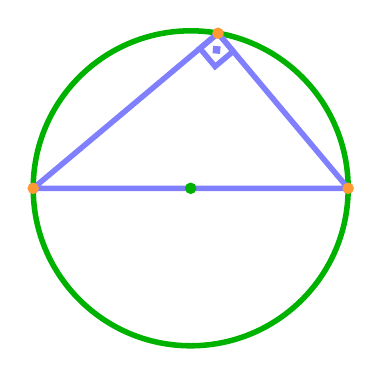
\begin{tikzpicture}
\tikzstyle{texto}=[draw=none,fill=none,black!60!white]
\tikzstyle{line2}=[blue!50!white,line width=2pt]
\tikzstyle{line}=[green!70!black,line width=2pt]
\tikzstyle{line3}=[orange!80!white,line width=2pt]
\tikzstyle{angleA}=[draw=none,fill=blue!50!white]
\tikzstyle{angleB}=[draw=none,fill=violet!30!white]

\draw[line] (0,0) circle (2);

\begin{scope}[shift={(80:2)}, rotate=-140]
    \draw[line2] (0,0) rectangle (0.3,0.3);
    \filldraw[line2] (0.15,0.15) circle (0.5pt);
\end{scope}

\draw[line2] (-2,0) -- (0:2) (-2,0) -- (80:2) -- (0:2);

\filldraw [line] (0,0) circle (1pt);
\filldraw [line3] ((-2,0) circle (1pt);
\filldraw [line3] (0:2) circle (1pt);
\filldraw [line3] (80:2) circle (1pt);

%\node[texto] at (1.9,-1.3) {\textbf{$\alpha$}};
%\node[texto] at (-1.7,-1.5) {\textbf{$\beta$}};
%\node[texto] at (-1.3,-0.2) {\textbf{$\alpha$}};
\end{tikzpicture}
\end{center}

\TM{Ângulos Inscritos}

A propriedade fundamental dos ângulos inscritos numa circunferência estabelece que todos os ângulos inscritos que subtendem o mesmo arco terão sempre a mesma medida, independentemente da posição de seus vértices na circunferência. Essa característica é crucial em geometria e trigonometria, sendo essencial para o estudo de círculos e polígonos inscritos.

\begin{center}
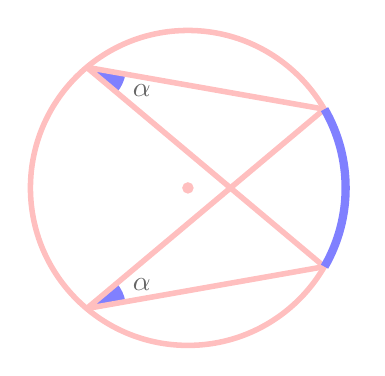
\begin{tikzpicture}
\tikzstyle{texto}=[draw=none,fill=none,black!60!white]
\tikzstyle{line}=[pink,line width=2pt]
\tikzstyle{line2}=[blue!50!white,line width=3pt]
\tikzstyle{angleA}=[draw=none,fill=blue!50!white]
\tikzstyle{angleB}=[draw=none,fill=blue!30!white]

\begin{scope}[shift={(230:2)}]
    \draw[angleA] (0,0) -- (10:0.5) arc (10:40:0.5);
    \node[texto] at (0.7,0.3) {\textbf{$\alpha$}};
\end{scope}

\begin{scope}[shift={(130:2)}]
    \draw[angleA] (0,0) -- (-40:0.5) arc (-40:-10:0.5);
    \node[texto] at (0.7,-0.3) {\textbf{$\alpha$}};
\end{scope}

\draw[line] (130:2) -- (30:2) (130:2) -- (-30:2);
\draw[line] (230:2) -- (30:2) (230:2) -- (-30:2) ;

\filldraw [line] (0,0) circle (1pt);
\draw[line] (0,0) circle (2);

\begin{scope}[shift={(1.735,-1)}]
    \draw[line2] (0,0) arc (-30:30:2);
\end{scope}

\end{tikzpicture}
\end{center}

\TM{Exemplo:}

\begin{center}
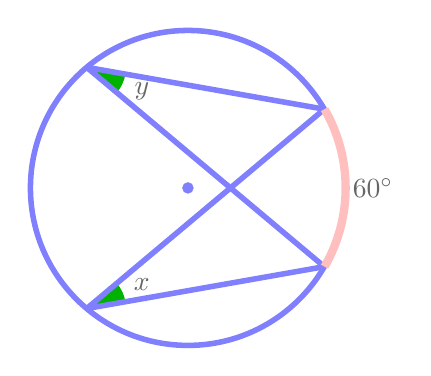
\begin{tikzpicture}
\tikzstyle{texto}=[draw=none,fill=none,black!60!white]
\tikzstyle{line}=[blue!50!white,line width=2pt]
\tikzstyle{line2}=[pink,line width=3pt]
\tikzstyle{angleA}=[draw=none,fill=green!70!black]
\tikzstyle{angleB}=[draw=none,fill=blue!30!white]

\begin{scope}[shift={(230:2)}]
    \draw[angleA] (0,0) -- (10:0.5) arc (10:40:0.5);
    \node[texto] at (0.7,0.3) {\textbf{$x$}};
\end{scope}

\begin{scope}[shift={(130:2)}]
    \draw[angleA] (0,0) -- (-40:0.5) arc (-40:-10:0.5);
    \node[texto] at (0.7,-0.3) {\textbf{$y$}};
\end{scope}

\draw[line] (130:2) -- (30:2) (130:2) -- (-30:2);
\draw[line] (230:2) -- (30:2) (230:2) -- (-30:2) ;

\filldraw [line] (0,0) circle (1pt);
\draw[line] (0,0) circle (2);

\begin{scope}[shift={(1.735,-1)}]
    \draw[line2] (0,0) arc (-30:30:2);
\end{scope}

\node[texto] at (2.35,0) {\textbf{$\ang{60}$}};

\end{tikzpicture}
\end{center}

Neste exemplo temos que $x=y$ pela propriedade dos ângulos inscritos.

\vspace{8px}
$x = \dfrac{60}{2} = 30$ \vspace{8px}

\TM{Diâmetro}

O diâmetro divide a circunferência em dois semicírculos de $\ang{180}$ cada. Se um ponto $P$ na circunferência forma os arcos $\alpha$ e $\beta$ com as extremidades do diâmetro, então esses dois arcos complementam o círculo inteiro:

\Formula{\alpha + \beta = \ang{180}}

\begin{center}
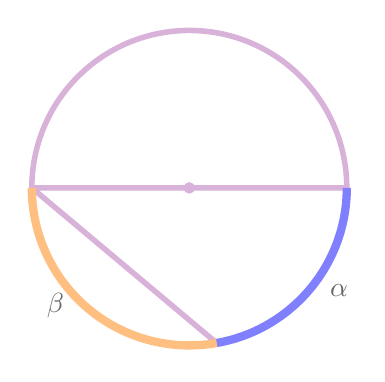
\begin{tikzpicture}
\tikzstyle{texto}=[draw=none,fill=none,black!60!white]
\tikzstyle{line}=[violet!30!white,line width=2pt]
\tikzstyle{line2}=[blue!50!white,line width=3pt]
\tikzstyle{line3}=[orange!50!white,line width=3pt]
\tikzstyle{angleA}=[draw=none,fill=blue!50!white]
\tikzstyle{angleB}=[draw=none,fill=violet!30!white]

\begin{scope}[shift={(-2,0)}]
   % \draw[angleA] (0,0) -- (-40:0.5) arc (-40:0:0.5);
\end{scope}

\draw[line] (-2,0) -- (0:2) (-2,0) -- (-80:2) ;

\filldraw [line] (0,0) circle (1pt);
\draw[line] (0,0) circle (2);

\begin{scope}[shift={(2,0)}]
    \draw[line2] (0,0) arc (0:-80:2);
\end{scope}
\begin{scope}[shift={(-2,0)}]
    \draw[line3] (0,0) arc (180:280:2);
\end{scope}

\node[texto] at (1.9,-1.3) {\textbf{$\alpha$}};
\node[texto] at (-1.7,-1.5) {\textbf{$\beta$}};
%\node[texto] at (-1.3,-0.2) {\textbf{$\alpha$}};
\end{tikzpicture}
\end{center}

\TM{Exemplo:}

\begin{center}
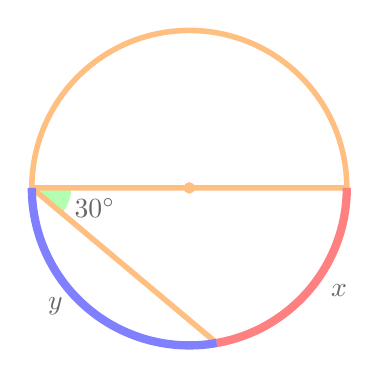
\begin{tikzpicture}
\tikzstyle{texto}=[draw=none,fill=none,black!60!white]
\tikzstyle{line}=[orange!50!white,line width=2pt]
\tikzstyle{line2}=[red!50!white,line width=3pt]
\tikzstyle{line3}=[blue!50!white,line width=3pt]
\tikzstyle{angleA}=[draw=none,fill=green!30!white]
\tikzstyle{angleB}=[draw=none,fill=violet!30!white]

\begin{scope}[shift={(-2,0)}]
   \draw[angleA] (0,0) -- (-40:0.5) arc (-40:0:0.5);
\end{scope}

\draw[line] (-2,0) -- (0:2) (-2,0) -- (-80:2) ;

\filldraw [line] (0,0) circle (1pt);
\draw[line] (0,0) circle (2);

\begin{scope}[shift={(2,0)}]
    \draw[line2] (0,0) arc (0:-80:2);
\end{scope}

\begin{scope}[shift={(-2,0)}]
    \draw[line3] (0,0) arc (180:280:2);
\end{scope}

\node[texto] at (1.9,-1.3) {\textbf{$x$}};
\node[texto] at (-1.7,-1.5) {\textbf{$y$}};
\node[texto] at (-1.2,-0.25) {\textbf{$\ang{30}$}};
\end{tikzpicture}
\end{center}

Pela propriedade do ângulo inscrito temos que:

\vspace{8px}
$30 = \dfrac{x}{2}$ \vspace{8px}

$\dfrac{x}{2} = 30$ \vspace{8px}

$x = 30 \cdot 2$

$x=60$

Pela propriedade do diâmetro, temos que:

$x+y=180$

$60+y=180$

$y=180-60$

$y=120$

\TM{Quadrilátero Inscrito}

Quando um quadrilátero tem todos os seus vértices sobre uma circunferência, dizemos que ele é um \textbf{quadrilátero inscrito}. Nesses quadriláteros, os ângulos opostos são sempre suplementares:

\Formula{A + C = \ang{180} \qquad B + D = \ang{180}}

Isso é consequência direta da propriedade do ângulo inscrito: cada par de ângulos opostos subtende arcos que juntos completam os \ang{360} da circunferência, portanto cada ângulo inscrito vale metade de \ang{360}, ou seja, \ang{180} somados.

\TM{Exemplo:}

Em um quadrilátero inscrito, três ângulos medem $\ang{80}$, $\ang{95}$ e $\ang{110}$. Qual é o quarto ângulo?

Usando $A + C = \ang{180}$ e $B + D = \ang{180}$:

\vspace{8px}
$\ang{80} + C = \ang{180}$ \quad $\Rightarrow$ \quad $C = \ang{100}$

$\ang{95} + D = \ang{180}$ \quad $\Rightarrow$ \quad $D = \ang{85}$

Verificação: $80 + 95 + 100 + 85 = \ang{360}$ \checkmark

\end{multicols}

\lfoot{\scriptsize © Copyright, Pratique Já}
\cfoot{\large \textcolor{bluebell}{pratiqueja.com}}
\end{document}